\section{Introduction}

\begin{frame}[allowframebreaks]
	\frametitle{Pourquoi ?}
	\begin{center}
		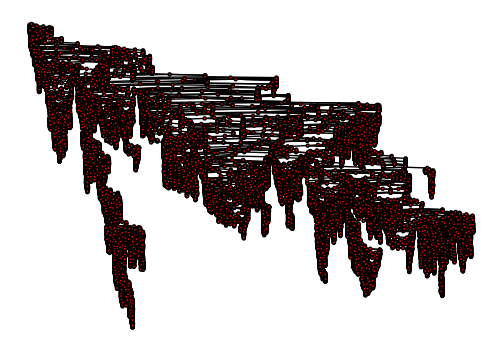
\includegraphics[width=7cm]{exempleIntro} \\
		\begin{itemize}
			\item Pourquoi des arbres ? Structure primordiale en informatique. 
			\item Pourquoi afficher des arbres de grande taille ? Pour observer des tendances. %répartition hauteur/largeur, forme générale, etc
		\end{itemize}
	\end{center}
\end{frame}

\begin{frame}
	\frametitle{Objectif}
	\begin{block}{Objectif du projet}
		Affichage élégant et efficace de tout type d'arbre
	\end{block}
	\begin{alertblock}{Problèmes}
		\begin{itemize}
			\item Qu'est-ce qu'un affichage élégant ?
			\item Comment optimiser le calcul de la mise en page ?
		\end{itemize}
	\end{alertblock}
\end{frame}


%Des outils existent actuellement pour représenter des arbres de grande taille de façon efficace. Citons par exemple GraphViz. L'inconvénient d'un tel outil est qu'il ne prend pas en compte l'ordre des fils. Ceci pose problème lorsque l'on souhaite représenter des arbres dont l'ordre des fils et primordial : les arbres de recherche.\\
%Ce projet consiste à fournir une alternative à Graphviz, afin de pouvoir visualiser n'importe quel type d'arbre, toujours de manière efficace, mais en conservant l'ordre des fils. Ce problème possède plusieurs problématiques. Tout d'abord, nous voulons que l'affichage d'un arbre soit faite de manière élégante. Ensuite, il faut que le calcul de la mise en page de l'arbre soit rapide.\\
%Pour ce faire, nous avons donc d\^u étudier les algorithmes déjà existants pour la mise en page élégante des arbres de grande taille. Sachant ces algorithmes, nous avons conçu un algorithme permettant cette mise en page. Enfin, nous avons implémenté cet algorithme, de telle façon qu'il puisse \^etre utilisé avec différentes sorties. Nous avons ici choisi de considérer trois sorties possibles : Tikz, pour pouvoir générer automatiquement un pdf ou intégrer le code à un document \LaTeX ; Asymptote, une alternative à Tikz ; et NetworkX, pour pouvoir générer une image de l'arbre que l'on pourra ultérieurement insérer dans n'importe quel document.
